% !TeX spellcheck = en_US

\chapter{Analysis}
The Analysis shows use-cases for the system based on the stakeholders. A gap-analysis is performed to compare use-cases of the new system in difference to the old one. The result of this process will be requirements, which are separated into functional and non-functional.


\section{Stakeholders}
Stakeholders are groups of people that have an interest in the system. This can be from a practical, or from a business standpoint. 

\subsection{Model Developer}
The Model Developer is a technical user that creates a MARS model in cooperation with a domain expert.

\subsection{Simulation Creator}
The Model Developer is an domain export. He Uses the Model, created by the Model Developer to answer a research question.

\subsection{Group Admin}
The Group Admin is a user of the system with a leading roll in his group. He wants to manage people belonging to a particular group and handle group dependent settings.

\subsection{Admin}
The Admin is a global acting user with far reaching permission inside the system.


\section{Use-cases}
The interaction with the system requires 7 main use-cases. These cases are following the central workflow, while 2 extra use-cases are for management purposes. Figure \ref{fig:use-cases} shows an overview.\\
This piece of work focuses on the highlighted area of the use-cases, which are described in the following paragraphs.
\begin{figure}[H]
	\centering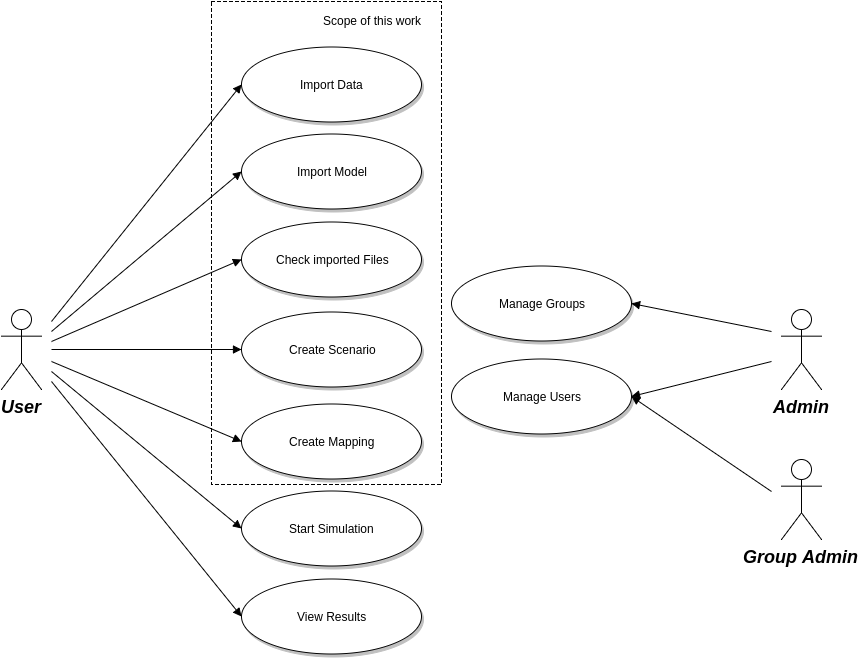
\includegraphics[width=1\textwidth]{res/Use-Cases}
	\caption{Use-Cases in UML notation}
	\label{fig:use-cases}
\end{figure}

\subsection{Import Data}
\begin{usecase}
	\addtitle{Name}{I: Import data}
	\addfield{Summary}{Upload local files to the Websuite, to use them for a simulation.}
	\additemizedfield{Actors}{
		\item Model Developer
		\item Simulation Creator
	}
	\additemizedfield{Preconditions}{
		\item Import data page is open.
	}
	\additemizedfield{Primary Scenario: }{
		\item The user drags one or multiple files onto the upload window, fills the form for every file and starts the import.
	}
	\additemizedfield{Alternative Scenario: }{
		\item The user clicks the upload Window, fills the form for every file and starts the import.
	}
\end{usecase}

\subsection{Import Model}
\begin{usecase}
	\addtitle{Name}{II: Import model}
	\addfield{Summary}{Upload local model files to the Websuite, to use them for a mapping.}
	\additemizedfield{Actors}{
		\item Model Developer
		\item Simulation Creator
	}
	\additemizedfield{Preconditions}{
		\item Import Model page is open.
	}
	\additemizedfield{Primary Scenario: }{
	\item The user drags one or multiple files onto the upload window, fills the form for every file and starts the import.
	}
	\additemizedfield{Alternative Scenario: }{
		\item The user clicks the upload Window, fills the form for every file and starts the import.
	}
\end{usecase}

\subsection{Check imported Data}
\begin{usecase}
	\addtitle{Name}{III: Check imported data}
	\addfield{Summary}{Make sure all the imported files from data- and model-import were processed correctly}
	\additemizedfield{Actors}{
		\item Model Developer
		\item Simulation Creator
	}
	\additemizedfield{Preconditions}{
		\item Data View page is open
		\item Files have been imported
	}
	\additemizedfield{Primary Scenario: }{
		\item The User views imported files, filters them by category or text input, sorts them by certain fields and displays the detailed metadata for one entry, by clicking on it.
	}
	\additemizedfield{Alternative Scenario: }{
		\item none
	}
\end{usecase}

\subsection{Create Scenario}
\begin{usecase}
	\addtitle{Name}{IV: Create scenario}
	\addfield{Summary}{Create a scenario based on a model and map the necessary fields.}
	\additemizedfield{Actors}{
		\item Model Developer
		\item Simulation Creator
	}
	\additemizedfield{Preconditions}{
		\item Create Scenario page is open
		\item A model has been uploaded.
	}
	\additemizedfield{Primary Scenario: }{
		\item The user clicks the "add Scenario" button. Inside the new modal, he fills the form, selects a model and saves the new scenario.
	}
	\additemizedfield{Alternative Scenario: }{
		\item none
	}
\end{usecase}

\subsection{Create Mapping}
\begin{usecase}
	\addtitle{Name}{Create Mapping}
	\addfield{Summary}{Combine the fields from the uploaded model with uploaded data.}
	\additemizedfield{Actors}{
		\item Model Developer
		\item Simulation Creator
	}
	\additemizedfield{Preconditions}{
		\item Create Mapping page is open
		\item Data has been imported
		\item Model has been imported
	}
	\additemizedfield{Primary Scenario: }{
		\item The user selects a scenario and starts mapping the required fields to a dataset. He than sets the parameters for the simulation.
	}
	\additemizedfield{Alternative Scenario: }{
		\item none
	}
\end{usecase}


\section{Gap-Analysis}


\section{Requirements}

\subsection{Functional Requirements}

\subsection{Non-Functional Requirements}
